\chapter{Systematic and statistical uncertainty calculations}
\label{chp:syst}



\section{Systematic uncertainty calculation methodology}


The systematic uncertainities for this analysis are calculated using the probablity distribution functions of each quantity appearing in the formula for the mean neutron multiplicity, which is given by:

\begin{equation}
    M=\frac{\# n_{\text {det }}-R \times \# \nu_{\text {det }}}{T} \frac{1}{\# \nu_{\text {det }}}
 \label{multiplicity}
\end{equation}



By random sampling the probability distribution functions for each of the terms in Equation \eqref{multiplicity} one can calculate the multiplicity probability distribution functions for both the statistical uncertainty and the systematic uncertainty. The statistical uncertainty for the value for the multiplicity is related to the variation in the number of detected neutrons, while the systematic uncertainty is related to the variation on the tagging efficiency and the background rate. The total search time for the tagged neutrons is dependent on the number of "windows" in which the neutron is searched for in, and therefore the term for the number of detected neutrinos. Because any variation on the number of neutrinos which are detected is unrelated to the value for the mean neutron multiplicity, calculating a probability mass function for the number of neutrinos is uneccessary. 

A Poissonian distribution is used to model the distribution for the number of detected neutrons, due to its value being approximated by counting the positives in the timing window that the neutron tagging search is carried out in. The mean value of this Poisson distribution is the number of detected neutrons $\left\langle \# n_{\text {detected}}\right\rangle$.
\newline
\begin{equation}
    P M F\left(\# n_{\text {detected}}\right)=\frac{1}{\left(\# n_{\text {detected}}\right) !}\left\langle \# n_{\text{detected }}\right\rangle^{\# n_{\text {detected}}} e^{-\left\langle \# n_{\text {detected}}\right\rangle}
\label{poissonuncertainty}
\end{equation}
\newline
Regarding the background rate, this is estimated from dummy spill data. The background rate error is associated with the statistical variation of the Monte Carlo size that the backround rate is associated with, and secondly the change of the background rate value during the SK-V period. The statistical variation of the MC is modelled using a Poisson, but the statistics are high enough so that it appears Gaussian, while the uncertainty relating to time variation is characterised by its own probability distribution function. In contrast, the tagging efficiency is model dependent and has systematic uncertainties relating to this. The two ways in which the systematic error are estimated are either using MC re-weighting or MC regeneration.
\newline
For the MC-reweighting approach, weights are applied to a quantity and the tagging efficiency of the re-weighted MC is extracted. The general methodology is to have the input of a model (given by a set of parameters) and to vary them one by one and then calculate the reweighted tagging efficiencies - the set of relative discrepancies $\delta_{i}$ are computed from this set of reweighted tagging efficiencies $T_{i}$ and the nominal tagging efficiency $T_{nom}$ using Equation \eqref{tageffdiscrep}.
\newline
\begin{equation}
    \delta_{i}=\frac{T_{i}-T_{\text {nom }}}{T_{\text {nom }}} \quad i \in\{\text { parameters }\}
\label{tageffdiscrep}
\end{equation}
\newline

These relative discrepancies $\delta_{i}$ are used to calculate the one indivdual discrepancy $\delta_{reweighted}$ that would describe the final deviation from the nominal tagging efficiency $T_{nom}$ due to the systematic error. The parameter $\delta_{reweighted}$ describes the model which has been produced through 1$\sigma$ variations of these parameters, therefore the final probability distribution function which describes the deviation from the nominal MC has a Gaussian distribution with the standard deviation being equal to $\delta_{reweighted}$. 
\newline
The other method to estimate the systematic error on the tagging efficiency is the method of Monte Carlo regeneration. This is carried out by varying a parameter then regenerating the whole Monte Carlo and then extracting the tagging efficiency - therefore unlike with MC re-weighting there is no set of discrepancies $\delta_{i}$ but instead two single discrepancies $\delta_{min}$ and $\delta_{max}$. The resulting probability distribution which describes the deviation from the nominal Monte Carlo is a Gaussian which has the mean and standard deviation relating to the discrepancies shown in Equation \eqref{mcregengauss}.
\newline

\begin{equation}
\left\{\begin{array}{l}
\mu=\frac{\delta_{\max }+\delta_{\min }}{2} \\
\sigma=\frac{\delta_{\max }-\delta_{\min }}{2}
\end{array}\right.
\label{mcregengauss}
\end{equation}


\section{Neutrino beam flux uncertainty}

The uncertainty on neutrino beam fluxes can be evaluated by looking at the dependence of the tagging efficiency on the flux variations. The beam fluxes for the four flavour modes 
$\left(\nu_{e} \overline{\nu_{e}} \nu_{\mu} \overline{\nu_{\mu}}\right)$ have the fractional uncertainties given for each mode, FHC and RHC. The binned uncertainties are shown in Figure \ref{fig:frac_beam_flux_uncertainty}.


Each individual bin for the flux is increased/decreased by its error, the Monte Carlo re-weighting method is then used to extract the taggging efficiency for each flux bin, and Equation \eqref{nubeamfluxerror} is used to calculate the fractional uncertainty.
\newline
\begin{equation}
    \delta_{i}(\pm \sigma)=\frac{T_{i}(\pm \sigma)-T_{\text {nom }}}{T_{\text {nom }}} \quad i \in\{\text { each flux bin }\}
\label{nubeamfluxerror}
\end{equation}
\newline
Figure \ref{fig:fluxuncertainty} shows the fractional errors calculated from the reweighted Monte Carlo, with the red bars showing the -1$\sigma$ variation and the blue bars showing the +1$\sigma$ variation. Table \ref{table:systuncertaintytable} contains the value for the total uncertainty resulting from the neutrino beam flux, which was calculated using Equation \eqref{summingfluxuncertainty}, where the maximum value between the increased and decreased discrepancy is taken and summed over to produce the final neutrino flux beam uncertainty.
\newline

\begin{figure}
    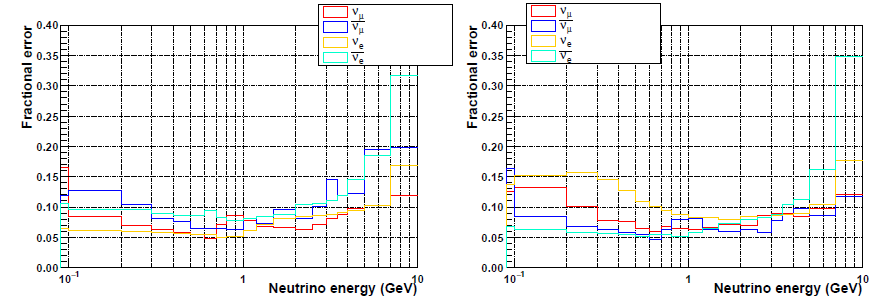
\includegraphics[width=\textwidth]{Figures/frac_beam_flux_uncertainty.png}
    \caption{Fractional uncertainties of beam fluxes.}
    \label{fig:frac_beam_flux_uncertainty}
\end{figure}


\begin{equation}
    \delta_{\nu \text { flux }}=\sum_{i \in\{\text { bins }\}} \max \left[\left|\delta_{i}(+\sigma)\right|,\left|\delta_{i}(-\sigma)\right|\right]
 \label{summingfluxuncertainty}   
\end{equation}

\begin{figure}
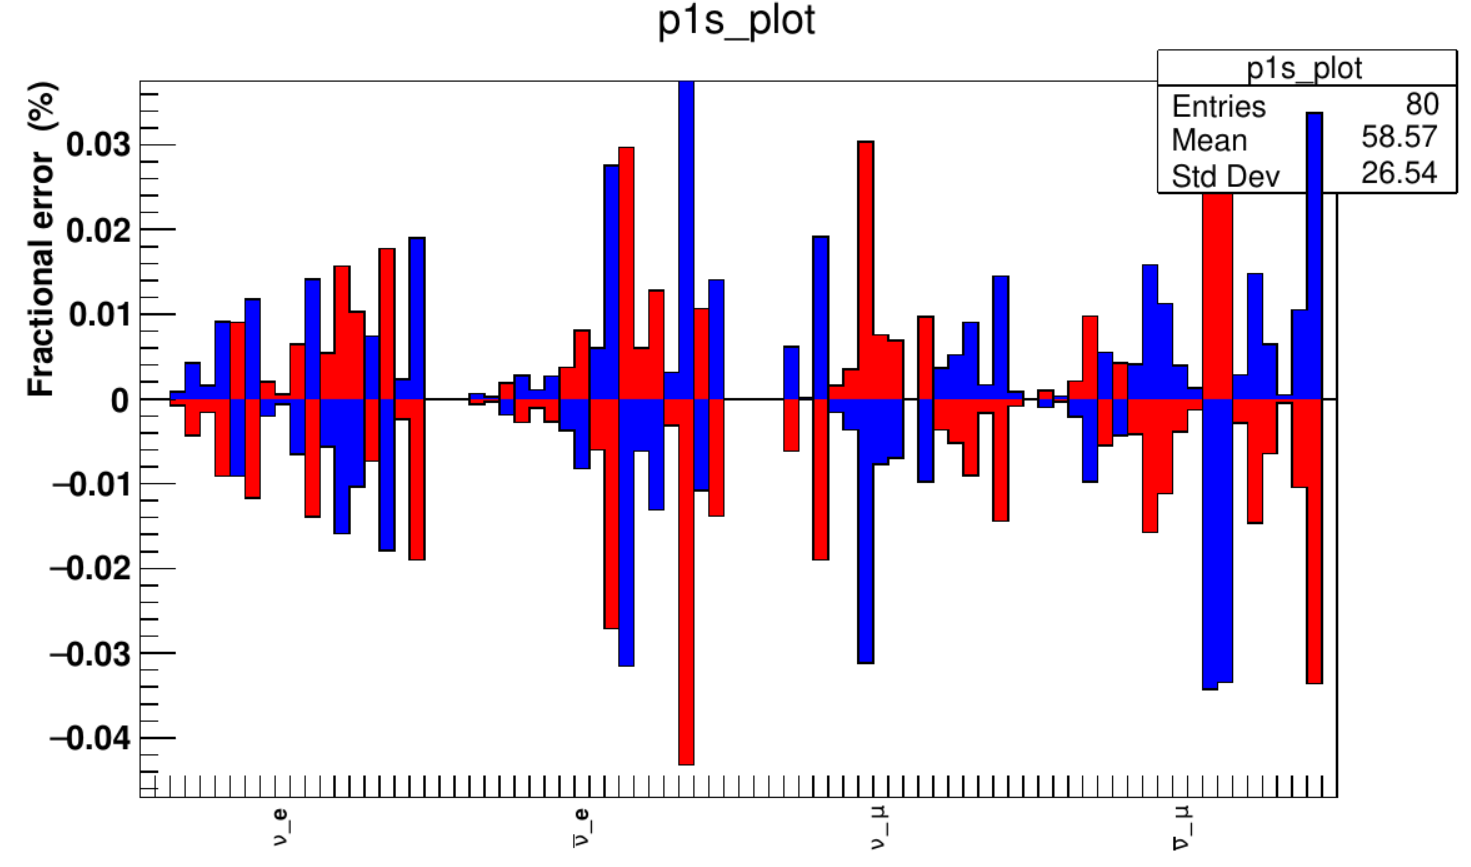
\includegraphics[scale=0.4]{Figures/flux_uncertainty.png}
\caption{Tagging efficiency fractional uncertainties caused by neutrino beam flux discrepancies. From left to right the sections in this plot are comprised of the beam fluxes elements of $\left(\nu_{e} \overline{\nu_{e}} \nu_{\mu} \overline{\nu_{\mu}}\right)$ respectively.}
\label{fig:fluxuncertainty}
\end{figure}

\section{Neutrino cross section uncertainty}

A group of default neutrino cross section values are used to make up the nominal Monte Carlo from which the tagging efficiency is calculated. The values of the parameters that determine the cross sections are shown in Table \ref{xsectable}. Each of the parameter values relate to a specific interaction type and are either a normalisation parameter or a paramater which shows a kinematic dependence. \newline

For charged current quasi-elastic interactions, the uncertainty is described by the Fermi momentum of the oxygen nucleus, ($p_{F}^{O}$), the binding energy of the oxygen nucleus,($E_{B}^{O}$) and the axial mass $M_{A}^{C C Q E}$. The axial mass for CCQE interactions relates to the axial form factor which along with vector form factors is proportional to the cross section of the interactions. For neutrino interactions where two nucleons produce two holes (2p2h), an overall normalisation parameter takes the uncertainty of these interactions into account. For $CC$ and $NC1\pi$ interactions, the uncertainty is described by the isospin background, the axial form factor $C_{A 5}^{R E S}$ which just like for CCQE interactions relates to the axial mass $M_{A}^{R E S}$. For neutral current and charged current interactions (both elastic and inelastic) there are normalisation parameters and energy dependent parameters to take the uncertainty into account. Finally, for charged current interactions with electron neutrinos, the braking radiation from the lepton in the final state is also considered when calculating the uncertainty and is treated using a normalisation parameter.
\newline

The Monte Carlo re-weighting method is used to reweight the nominal Monte Carlo on an event by event basis with each parameter value being increased and decreased by its uncertainty, and for each reweighted Monte Carlo the equivalent tagging efficiency value is extracted. Equation \eqref{xsectageff} shows how the fractional discrepancies are extracted from the nominal and reweighted tagging efficiency values.

\begin{equation}
\delta_{i}(\pm \sigma)=\frac{T_{i}(\pm \sigma)-T_{\text {nom }}}{T_{\text {nom }}} \quad i \in\{\text { parameters }\}
\label{xsectageff}
\end{equation}

Figure \ref{fig:xsecuncertainty} shows the reweighted Monte Carlo fractional uncertainty plotted for the FHC sample. Since this sample contains a lot of NCother interactions, the uncertainty for this interaction type is greater than for the others.

\begin{table}
    \centering
        $\begin{array}{||cccc||}
        \hline & & & \\
        \text { Parameter } & \text { Interaction } & \text { Type } & \text { Value } \\
        \hline & & & \\
        p_{F}^{O} & \text{CCQE} & { }^{16} \text{O} \text { Fermi momentum } & 225 \pm 31 \text{MeV} / \text{c} \\
        E_{B}^{O} & \text{CCQE} & { }^{16} \text{O} \text { binding energy } & 27 \pm 9 \text{MeV} \\
        M_{A}^{C C Q E} & \text{CCQE} & \text { Axial mass } & 1.2 \pm 0.41 \text{GeV} / \text{c}^{2}\\
        2 p 2 h & 2 \text{p} 2 \text{~h} & \text { Normalization par. } & 1.0 \pm 1.0 \\
        C_{A 5}^{R E S}& \text{CC} \text { and } \text{NC} 1 \pi & \text { Axial form factor } & 1.01 \pm 0.12 \\
        M_{A}^{R E S}  & \text{CC} \text { and NC1 } \pi & \text { Axial mass } & 0.95 \pm 0.15 \text{GeV} / \text{c}^{2} \\
        B G_{A}^{R E S} & \text{CC} \text { and } \text{NC} 1 \pi & \text{I}=1 / 2 \text { continuum background } & 1.3 \pm 0.2 \\
        \text{CC} \text { other } & \text{CC} \text { other } & \text { E-dependent par. } & 0.0 \pm 0.4 \\
        \text{CC} \text { elastic } & \text{CC} \text { elastic } & \text { Normalization par. } & 1.0 \pm 0.3 \\
        \text{NC} \text { other } & \text{NC} \text { other } & \text { E-dependent par. } & 1.0 \pm 0.3 \\
        \text{NC} \text { elastic } & \text{NC} \text {  elastic } & \text { Normalization par. } & 1.0 \pm 0.3 \\
        \text{FS} e^{-} \text {Bremsstrahlung } & \text{CC} \nu_{e} & \text { Normalization par. } & 1.00 \pm 0.03 \\
        \hline
        \end{array}$
        \caption{Neutrino cross section parameters}
        \label{xsectable}
\end{table}


\begin{figure}
    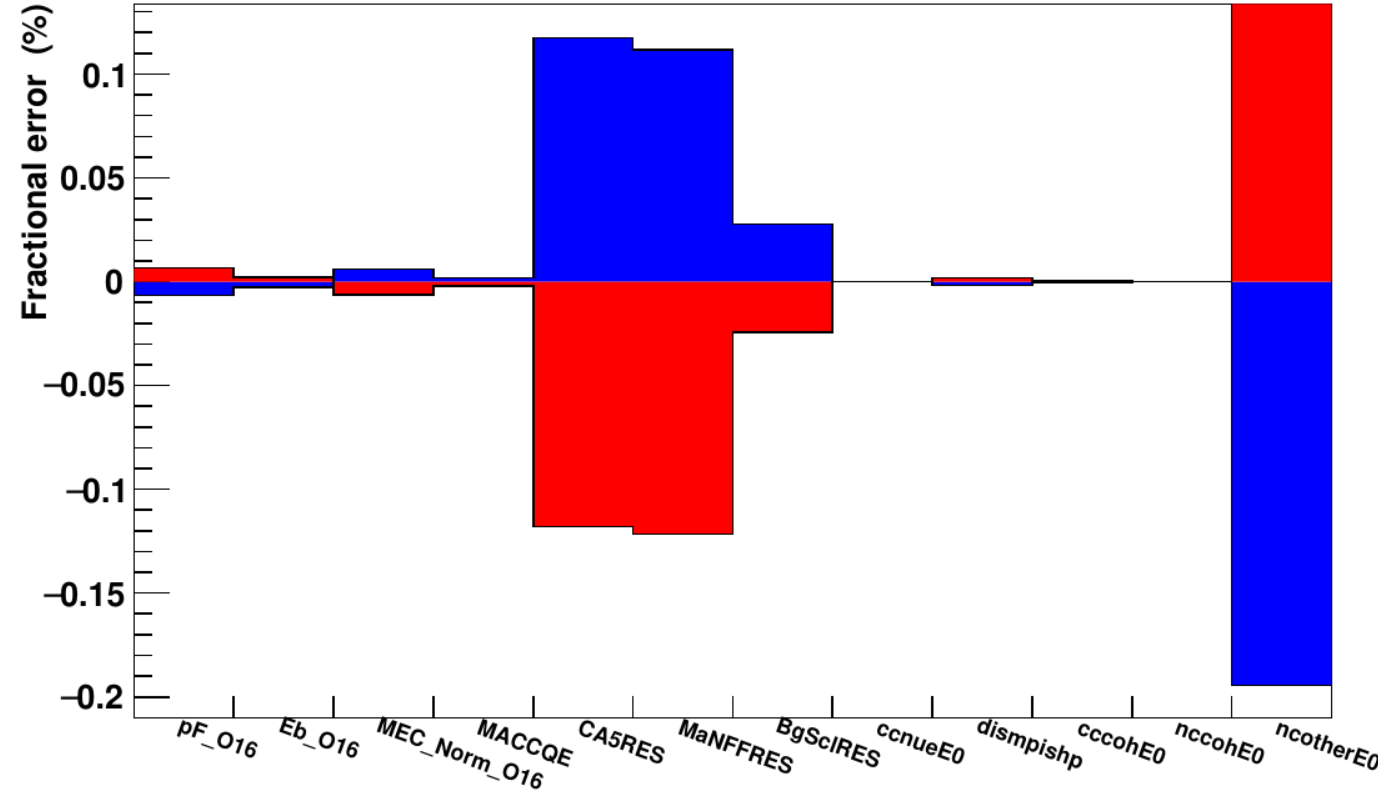
\includegraphics[scale=0.4]{Figures/xsec_uncertainty.png}
\caption{Tagging efficiency uncertainty caused by the cross-section parameters variations for the FHC mode}
\label{fig:xsecuncertainty}
\end{figure}

\section{Pion final state interaction (FSI) and secondary interaction (SI) uncertainties}

Even though this is an analysis concerned with neutral current quasi elastic interactions, pion events are a significant contribution to the background, and as a result it is important to examine the pion interaction uncertainties both for final state interactions and secondary interactions as their trajectories span the detector. 
\newline


The neutrino-nucleus interaction simulator used in this analysis (NEUT) handles pion final state interactions and secondary interactions using a cascade model. This cascade model contains parameters which will have uncertainties on them and these will be tranferred to a possible change in the tagging efficiency.

Depending on the momentum of the pions, different interaction types occur in the model. For pions with a momentum less than 500 MeV, the interactions in place are absorption (ABS), quasi-elastic scattering (QE) and charge exchange (CX).

Absorption occurs when the incident pion is absorbed by the nucleus and no pions remain in the final state. Quasi-elastic (QE) scattering occurs when there is only one pion observed in the final state and it has the same charge as the incident beam. Charge exchange occurs when the charged pion interacts wtht he nucleus and a single $\pi_{0}$ can be seen in the final state.


For pions with a momentum of greater than 500 MeV, a different set of interactions are used. Inelastic interactions (INEL) can now produce hadrons and replace absorption processes, but quasi-elastic scattering (QEH) and charge exchange (CXH) will still occur. The final state interaction parameters and the pion momentum range they are used in can be seen in Table \ref{fsiparameters}. Each parameter scales the relevant very small proabability of the charged pion interaction at every stage of the intra-nuclear cascade, aside from the parameter for charge exchange which scales only the fraction of low momentum QE scattering. 


\begin{table}
$$
\begin{array}{ccc}
\text { Parameter } & \text { Description } & \begin{array}{c}
\text { Momentum } \\
\text { Region }(\mathrm{MeV} / c)
\end{array} \\
f_{\mathrm{ABS}} & \text { Absorption } & <500 \\
f_{\mathrm{QE}} & \text { Quasi-elastic scatter } & <500 \\
f_{\mathrm{CX}} & \text { Single charge exchange } & <500 \\
f_{\mathrm{QEH}} & \text { Quasi-elastic scatter } & >500 \\
f_{\mathrm{CXH}} & \text { Single charge exchange } & >500 \\
f_{\mathrm{INEL}} & \text { Hadron }(\mathrm{N}+\mathrm{n} \pi) \text { production } & >500 \\
\end{array}
$$
\caption{Table showing the pion final state interaction parameters in NEUT and the pion momentum range they are used in}
\label{fsiparameters}
\end{table}
A set of paramater variations which determine a surface in paramater space have been estimated by pion scattering experiments, the values for which are shown in Table \ref{fsimodelparameters}. The 1$\sigma$ surface has been explored using the nominal Monte Carlo re-weighting method and the analagous tagging efficiency uncertainty is shown in Equation \ref{fsisitageff}, and the uncertainty stemming from the models shown in Table \ref{fsimodelparameters} is shown in Figure \ref{fig:fsisiuncertainty}

\begin{equation}
\delta_{i}=\frac{T_{i}-T_{\text {nom }}}{T_{\text {nom }}} \quad i \in \text { parameter vector }
\label{fsisitageff}
\end{equation}

\begin{figure}
    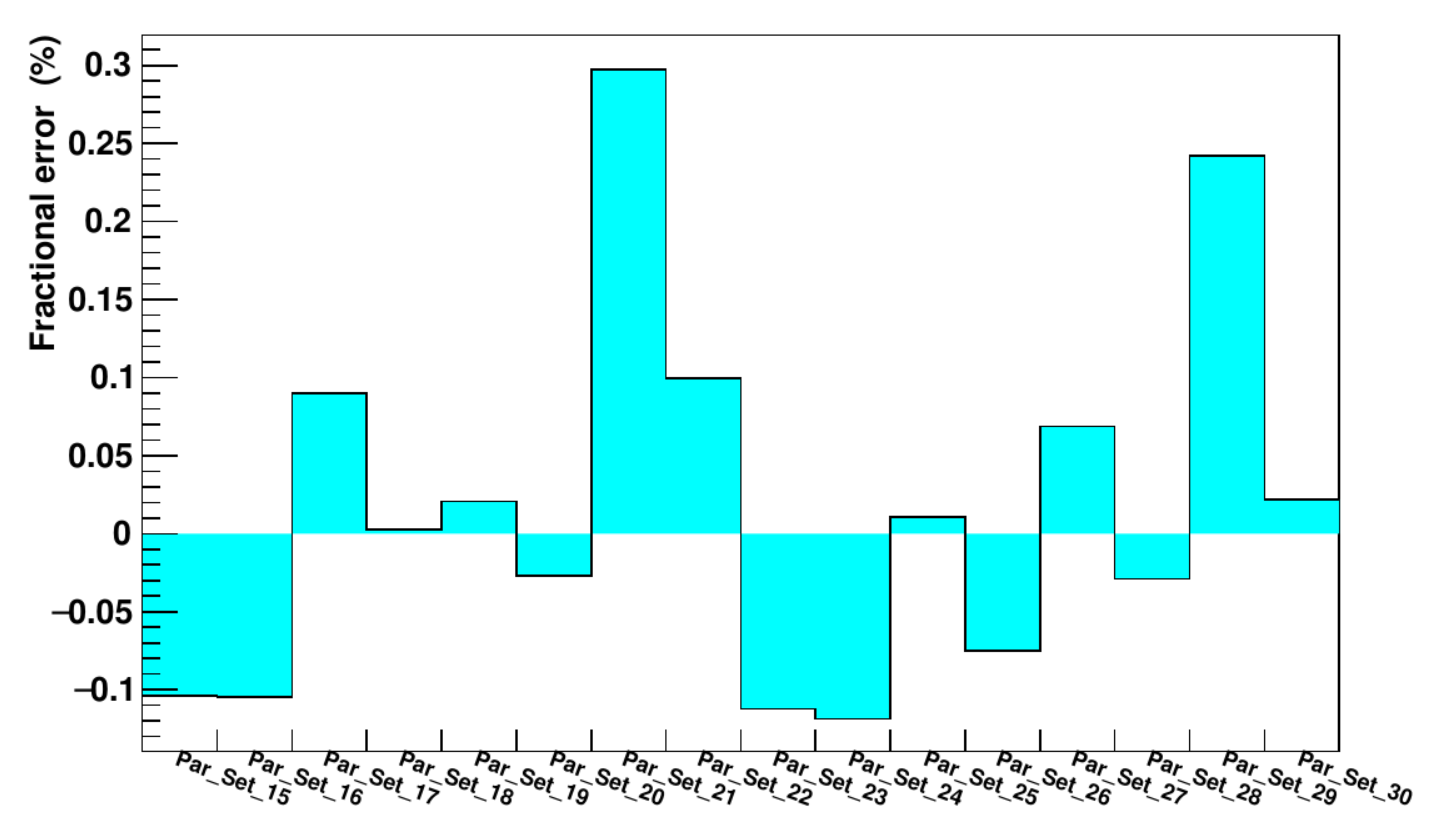
\includegraphics[scale=0.4]{Figures/fsisi_uncertainty.png}
\caption{Tagging efficiency fractional uncertainty caused by the variation in the FSI/SI model parameters for the FHC mode.}
\label{fig:fsisiuncertainty}
\end{figure}

\begin{table}
    $$
    \begin{array}{lllllll}
         & & & & & & \\
        \text { Set } & \text { ABS } & \text { QE } & \text { CX } & \text { INEL } & \text { QEH } & \text { CXH } \\
 %       \hline
    %\begin{array}{ccccccc}
    \text { Nominal } & 1.1 & 1.0 & 1.0 & 1.0 & 1.8 & 1.8 \\
    & & & & & & \\
    & 0.7 & 0.6 & 0.5 & 1.5 & 1.1 & 2.3 \\
    & 0.7 & 0.6 & 1.6 & 1.5 & 1.1 & 2.3 \\
    \text { Hadron production Up } & 1.6 & 0.7 & 0.4 & 1.5 & 1.1 & 2.3 \\
    & 1.6 & 0.7 & 1.6 & 1.5 & 1.1 & 2.3 \\
    & 0.6 & 1.4 & 0.6 & 1.5 & 1.1 & 2.3 \\
    & 0.7 & 1.3 & 1.6 & 1.5 & 1.1 & 2.3 \\
    & 1.5 & 1.5 & 0.4 & 1.5 & 1.1 & 2.3 \\
    & 1.6 & 1.6 & 1.6 & 1.5 & 1.1 & 2.3 \\
    & & & & & & \\
    & 0.7 & 0.6 & 0.5 & 0.5 & 2.3 & 1.3 \\
    & 0.7 & 0.6 & 1.6 & 0.5 & 2.3 & 1.3 \\
    & 1.6 & 0.7 & 0.4 & 0.5 & 2.3 & 1.3 \\
    \text { Hadron production Down } & 1.6 & 0.7 & 1.6 & 0.5 & 2.3 & 1.3 \\
    & 0.6 & 1.4 & 0.6 & 0.5 & 2.3 & 1.3 \\
    & 0.7 & 1.3 & 1.6 & 0.5 & 2.3 & 1.3 \\
    & 1.5 & 1.5 & 0.4 & 0.5 & 2.3 & 1.3 \\
    & 1.6 & 1.6 & 1.6 & 0.5 & 2.3 & 1.3
    \end{array}
    $$
\caption{Pion FSI/SI model parameter nominal value and variations grouped according to inelastic hadron production value}
\label{fsimodelparameters}
\end{table}

\section{Nucleon final state interactions}

Uncertainties regarding the nucleon final state interactions can change the number of nucleons knocked out of $\ch{^{16}O}$, therefore how the tagging efficiency is changed due to the variation in nucleon final state interactions needs to be investigated. This uncertainty is extracted using GENIE, a Monte Carlo event generator which contains the INTRANUKE (hA) intranuclear transport model. The uncertainties in the in the total scattering probability for hadrons inside the target nuclei ($x_{m f p}^{N}$) and the uncertainties in the likelihood of each hadron rescattering method: (elastic ($x_{e l}^{N}$), inelastic ($x_{i n e l}^{N}$), charge exchange ($x_{c e x}^{N}$), pion production ($x_{\pi}^{N}$) and absorption ($x_{a b s}^{N}$)) are taken into account. The fractional uncertainties for these modes for pions is shown in Table \ref{nucleonfsiuncertainties}. 

\begin{table}
$$
\begin{array}{llc}
\text {Abbreviation} & \text { Description of uncertainty }  & \text{Fractional uncertainty} \\
 x_{m f p}^{N} & \text { Nucleon mean free path (total rescattering probability) } & \pm 20 \% \\
x_{c e x}^{N} & \text { Nucleon charge exchange probability } & \pm 50 \% \\
x_{e l}^{N} & \text { Nucleon elastic reaction probability } & \pm 30 \% \\
x_{i n e l}^{N} & \text { Nucleon inelastic reaction probability } & \pm 40 \% \\
x_{a b s}^{N} & \text { Nucleon absorption probability } & \pm 20 \% \\
x_{\pi}^{N} & \text { Nucleon } \pi \text {-production probability } & \pm 20 \%
\end{array}
$$
\caption{Nucleon final state interaction parameters of the hA model executed inside GENIE.} 
\label{nucleonfsiuncertainties}
\end{table}

A nominal GENIE Monte Carlo sample is generated (different from the previously used NEUT Monte Carlo) and this shifted using the re-weighting method to a varied GENIE Monte Carlo by individually increasing and decreasing the parameters in Table \ref{nucleonfsiuncertainties} by its error. For each shifted Monte Carlo produced, the fractional uncertainty can be written as in Equation \ref{nucleonfsitageff}.

\begin{equation}
\delta_{i}(\pm \sigma)=\frac{T_{i}(\pm \sigma)-T_{\text {nom }}}{T_{\text {nom }}} \quad i \in\{\text { parameters }\}
\label{nucleonfsitageff}
\end{equation}

The tagging efficiency fractional uncertainties are displayed in Figure \ref{fig:nucleonfsiuncertainty}, showing which parameter from Table \ref{nucleonfsiuncertainties} each uncertainty has arisen from.

\begin{figure}
    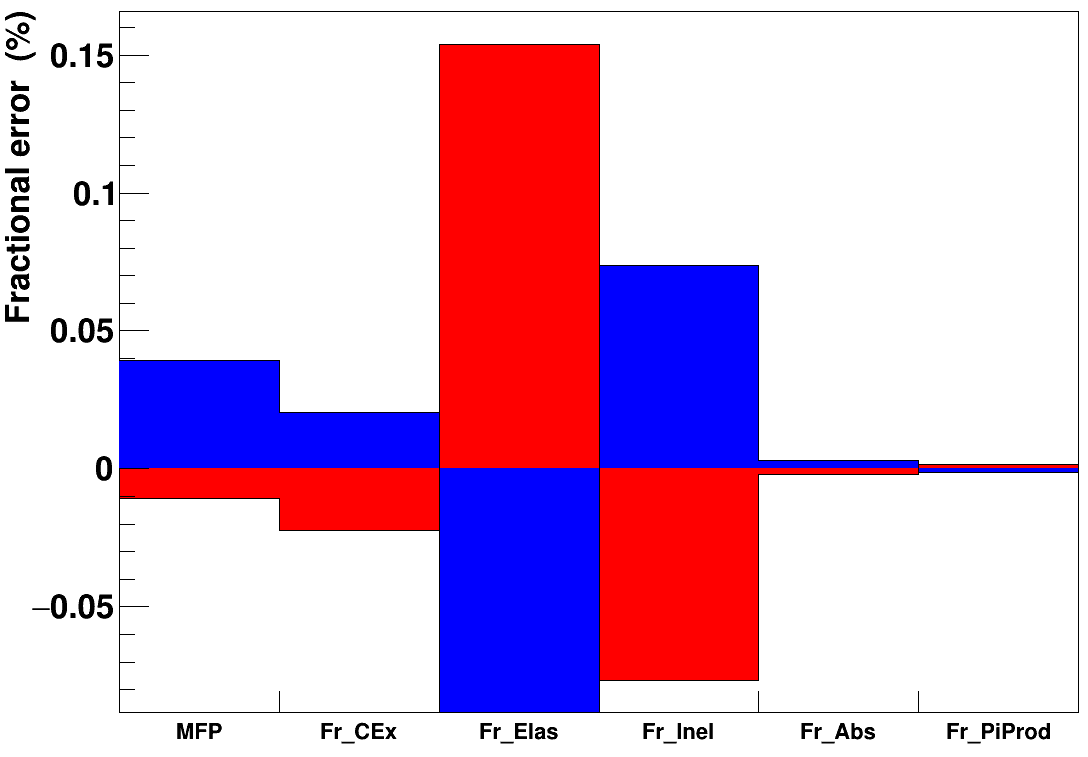
\includegraphics[scale=0.4]{Figures/nucleonfsi_uncertainty.png}
\caption{Tagging efficiency fractional uncertainties caused by the nucleon final state interaction model parameter variation for the FHC mode}
\label{fig:nucleonfsiuncertainty}
\end{figure}

\section{Muon and pion capture on Oxygen-16}

Neutrons are produced from negative muon capture on $\ch{^{16}O}$ as show in Equation \ref{muoncap}.

\begin{equation}
        \mu^{-}\;\ch{^{16}{O}}\;\longrightarrow\;\nu_{\mu}\;n\;\ch{^{15}{N}}
\label{muoncap}
\end{equation}

Direct neutrons are produced from pion capture on $\ch{^{16}O}$, but also a number of evaporation neutrons that leave the nucleus. For the capture of muons and pions on $\ch{^{16}O}$, the energy spectra of the neutrons produced have been measured: for muons the spectra can range up to 15 MeV, while in the case of pions the spectra can reach up to 100 MeV.


Geant4 simulates the capture processes for muons and pions, but there are alternate models that can be used: for example, the Chiral Invariant Phase Space (CHIPS) model for muon captures (based on non pertubative QCD) and two different routines for pion capture, one which is based on CHIPS and one based on intra-nuclear cascade.

Because any change in the model can alter the energy spectra of the neutrons, these alternative functions can be used to estimate the fractional uncertainties for the tagging efficiency. This is done by using the MC regeneration method, where the nominal Monte Carlo is regenerated by replacing the default Geant4 routines with the alternative models. For the alterantive muon capture model and the two alternative pion capture models, the fractional discrepancies are shown in Equation \ref{muoncaptaggingeff}.

\begin{equation}
    \begin{aligned}
        \delta_{muon C H I P S} &=\frac{T_{muon C H I P S}-T_{n o m}}{T_{\text {nom }}} \\
        \delta_{pion C H I P S} &=\frac{T_{pion C H I P S}-T_{n o m}}{T_{\text {nom }}} \\
        \delta_{pion B e r t} &=\frac{T_{pion B e r t}-T_{n o m}}{T_{\text {nom }}}
        \end{aligned}
        \label{muoncaptaggingeff}
\end{equation}

Figure \ref{fig:mupicap_uncertainty} shows the fractional uncertainties caused by muon and pion capture on oxygen for each model.

\begin{figure}
    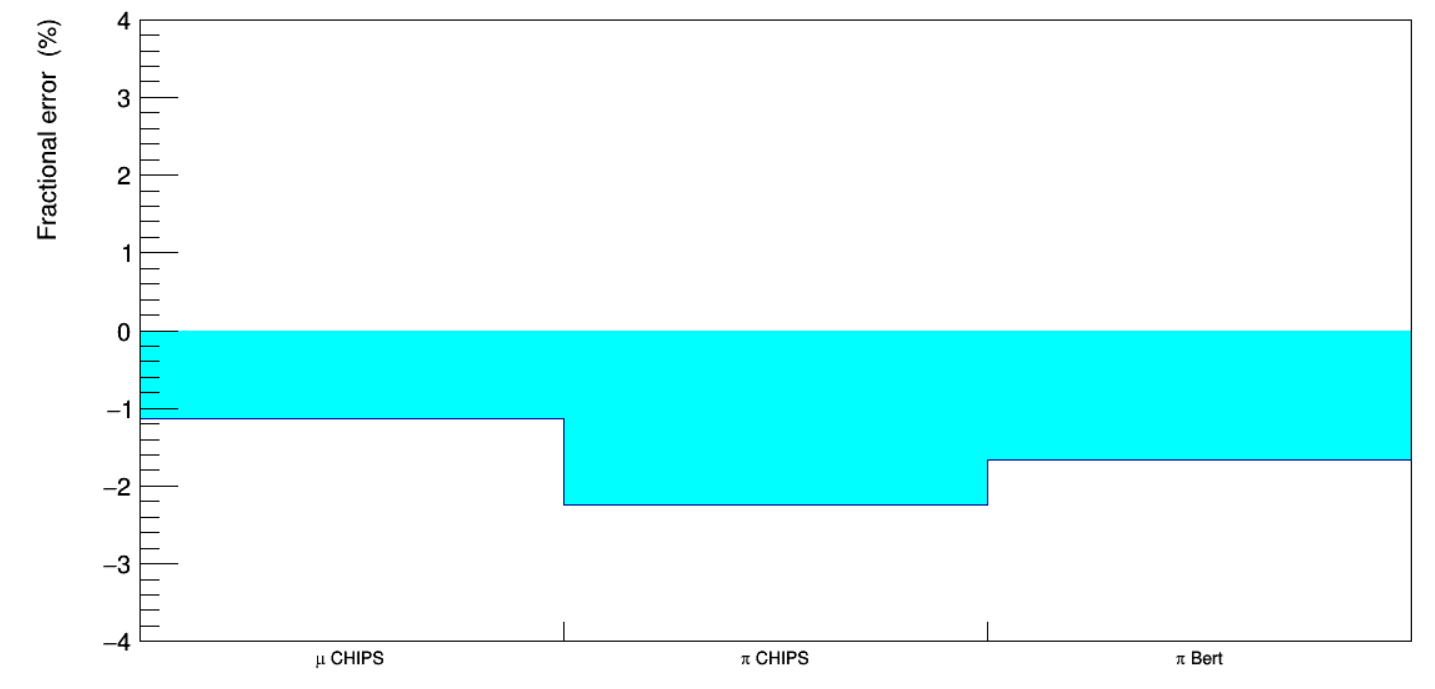
\includegraphics[scale=0.4]{Figures/mupicap_uncertainty.png}
\caption{Fractional uncertainties in the tagging efficiency caused by muon and pion capture on the muon capture CHIPS model, pion capture CHIPS model and the pion capture Bertini model.}
\label{fig:mupicap_uncertainty}
\end{figure}

\section{Nucleon SI}
Uncertainties in how Nucleon SI interactions are modelled can affect the tagging efficiency, due to how these uncertainties can affect the final number of nucleons present in the simulation and how far they travel in the detector medium. There are two Monte Carlo code systems used in order to determine how nucleons travel in the simulation, MICAP and HETC. These come as part of GCALOR, used to determine the energy and direction of incident hadrons, leptons and photons. MICAP (Monte-carlo-Ionization-Chamber-Analysis-Program), which simulates interactions based on calculated cross section and angular distributions for secondary particles, and is called for neutrons with a kinetic energy below 20 MeV. HETC on the other hand, is the High-Energy-Transport-Code, and is responsible for transporting charged hadrons above 20 MeV (up to an energy of 10 GeV) through the detector medium. 

\subsection{MICAP uncertainty calculation}

A library of cross-section data called ENDF (Evaluated Nuclear Data Files) are used by MICAP to determine what processes the neutrons go through in the detector medium, and their respective cross sections. There are two versions of libraries which are used in evaluating the uncertainty in the tagging efficiency, version B release V (released in 1978) and version B release VIII, released in 2018. There is very little difference between the total neutron on hydrogen cross sections between the two versions of the code, however, in the energy range of 0.1 MeV to 20 MeV, there are differences of up to 40\% in the cross-sections of neutron on oxygen cross sections. Both an elastic and inelastic part comprise the total cross-section of a nucleus, and these can effect the way neutrons travel in the simulated detector medium and also the way secondary particles from these interactions are distributed. The way these inelastic processes are simulated depend on the nuclei involved: hydrogen nuclei capture the neutrons in the range ($10^{-11}$, $10^{-7}$) MeV, while neutron captures on oxygen mainly happen n the 4 MeV to 20 MeV energy region.  To calculate the way uncertainties arise from the way MICAP simulates neutron captures, the ENDF-V library is replaced by ENDF-VIII, and the tagging efficiency using this library ($T_{VIII}$) is evaluated from regenerated MC. Equation \ref{eq:MICAP_uncertainty} shows the fractional uncertainty $\delta_{MICAP}$ regarding MICAP.  

\begin{equation}
    \delta_{m c p}=\frac{T_{V I I I}-T_{n o m}}{T_{n o m}}
\label{MICAP_uncertainty}
\end{equation}

\subsection{HETC uncertainty calculation}

Due to there being no experimental data for cross-section calculations on nucleon-oxygen scattering in the energy range at which T2K functions, experimental data of proton-carbon scattering is used to assign error on the cross sections. In the proton-carbon scattering analysis, NEUT was used to evaluate the theoretical cross sections of carbon, and this uses cross sections calculated using the Bertini model, which is also used in HETC. The comparison of these calculated cross sections to other theoretical calculations as well as to data, showed that the total cross sections calculated by Bertini need to varied by $\pm$ 30\% in order to be consistent with them. As a result of this, the Monte Carlo is regenerated twice where the free nucleon-nucleon cross sections are scaled by $\pm$ 30\%. Equation \ref{HETC_uncertainty} shows the fractional uncertainty $\delta_{HETC}(\pm)$, related to the corresponding tagging efficiencies ($T_{HETC}(\pm)$. 

\begin{equation}
    \delta_{HETC }(\pm)=\frac{T_{HETC}(\pm)-T_{nom }}{T_{nom }}
\label{HETC_uncertainty}
\end{equation}

\section{Uncertainty due to PMT gain simulation}

The change in PMT gain over time in the Super-K detector provides a systematic uncertainty to the simulations in this analysis. In SKDETSIM-SKGd the PMT gain drift is modelled by scaling the charge recieved by the PMT according to Equation \ref{eq:PMT_drift_gain}, where $G_{0}$ is the amount of average PMT gain value from October 2008. 

\begin{equation}
    Q \longrightarrow Q \times\left(1+\frac{G(t)-G_0}{G_0}\right)
\label{eq:PMT_drift_gain}
\end{equation}

In addition to the gain changing over time, so does the number of PMT hits due to the gain, and this has to be adjusted by a correction factor of $\alpha$ which has a value of 1.6, shown in Equation \ref{eq:PMT_drift_gain_scaling}. This value is estimated by comparing calibration data and simulations \cite{linyan_thesis}. For $alpha$ = 1, Equation \ref{eq:PMT_drift_gain_scaling} reduces to Equation \ref{eq:PMT_drift_gain}


\begin{equation}
    Q \longrightarrow Q \times\left(1+\alpha\frac{G(t)-G_0}{G_0}\right)
\label{eq:PMT_drift_gain_scaling}
\end{equation}

The discrepancies in tagging efficiency for this systematic uncertainty are produced by looking at the fractional uncertainty in tagging efficiencies between $\alpha$ = 1.6 and $\alpha$ = 1, according to Equation \ref{eq:PMT_gain_drift_uncertainty}.

\begin{equation}
    \delta_i=\frac{T_i^{\alpha=1.6}-T_i^{\alpha=1}}{T_i^{\alpha=1}} \quad i \in\{\text { Regeneration points }\}
\label{eq:PMT_gain_drift_uncertainty}
\end{equation}

This fractional discrepancy is calculated for each MC regeneration point and confidence bands are produced. In the range of the confidence band, millions of values are drawn from these confidence bands and the mean of these values is used as representation of the difference that occurs due to using $\alpha$ = 1.6 instead of $\alpha$ = 1. 

\section{Neutron oscillation uncertainty}

The tagging efficiency can also be altered by the uncertainty on the oscillation parameters. Using the oscillation parameters taken from TN-364, shown in Table \ref{table:nu_osc_params}, this tagging efficiency discrepancy is calculated. 

\begin{table}
    $$
    \begin{array}{llc}
         \text { Oscillation parameter } & \text { Value } \\
        \sin ^2 \theta_{13} & 0.0211 \pm 0.0008 \\
        \sin ^2 \theta_{23} & 0.541_{-0.037}^{+0.027} \\
        \left|\Delta m_{32}^2\right| & 2.469_{-0.071}^{+0.073} \times 10^{-3} \mathrm{eV}^2 \\
    \end{array}
    $$
\caption{Neutrino oscillation parameters.} 
\label{table:nu_osc_params}
\end{table}


For each of the oscillation parameters in Table \ref{table:nu_osc_params}, the nominal Monte Carlo is rewighted into two seperate new Monte Carlo outputs and which are produced after increasing or decreasing ($\pm$) the parameter in question by its errors. The related tagging efficiencies are extracted with their fractional uncertainties, given in Equation \ref{eq:osc_tageff_uncertainty}.   

\begin{equation}
    \delta_i(\pm \sigma)=\frac{T_i(\pm \sigma)-T_{\text {nom }}}{T_{\text {nom }}} \quad i \in\{\text { oscillation parameters }\}
\label{eq:osc_tageff_uncertainty}
\end{equation}

Due to the oscillation parameter uncertainties reflecting solely the oscillation probability error, this only affects the fraction of chrged current events in the sample, and because of this the resulting error is the smallest of the entire analysis. The tagging efficiency uncertainties for each oscillation parameter are summed together, with the maximum between the uncertainty values being taken as the total error, shown by Equation \ref{eq:final_osc_taggeff_uncertainty}.

\begin{equation}
    \delta_{\nu o s c}=\sum_i \max \left[\left|\delta_i(+\sigma)\right|,\left|\delta_i(-\sigma)\right|\right]
    \label{eq:final_osc_taggeff_uncertainty}
\end{equation}

\section{Uncertainty in detector response for neutrino events}

For neutrino events, it is the parameters produced by the Bonsai neutrino vertex fitter which encapsulates the detector response to neutrino events, specifically the reduction parameters $E_{rec}$, $ovaQ$, $\theta_{C}$ and paramaeters relating to position $dwall$ and $effwall$. As mentioned previously, cuts on the reduction variables are used to select the NCQE sample.

\subsection{Uncertainty on $E_{rec}$, $ovaQ$ and $\theta_{C}$}

The uncertainty on the $E_{rec}$, $ovaQ$ and $\theta_{C}$ parameters can alter the amount of NCQE events in the Monte Carlo and as a result, affect the tagging efficiency. TN-374 discusses the errors on these parameters \cite{tn_374} and are shown in Table \ref{table:erec_ovaq_thetac_errors}. 

\begin{table}
    $$
    \begin{array}{llc}
    \hline \text { Reduction parameter } & \text { Description } & \text { Uncertainty } \\
    \hline E_{\text {rec }} & \text { Reconstructed energy } & \pm 5 \% \\
    \text { ovaQ } & \text { Vertex and angular goodness coefficient } & \pm 1.5 \% \\
    \theta_C & \text { Cherenkov angle } & \pm 2 \text { degree } \\
    \hline
    \end{array}
    $$
\caption{Errors on the $E_{rec}$, $ovaQ$ and $\theta_{C}$ parameters} 
\label{table:erec_ovaq_thetac_errors} 
\end{table}

For each of these parameters, the nominal Monte Carlo is re-weighted into two new Monte Carlo outputs ($\pm$) and the related tagging efficiencies are extracted, where the fractional tagging uncertainty is shown in Equation \ref{eq:erec_ovaq_thetac_tageff}. 

\begin{equation}
    \delta_i(\pm \sigma)=\frac{T_i(\pm \sigma)-T_{\text {nom }}}{T_{\text {nom }}} \quad i \in\{\text { reduction parameters }\}
\label{eq:erec_ovaq_thetac_tageff}
\end{equation}


\subsection{Uncertainty on $dwall$ and $effwall$}

The neutrino vertex produced by the Bonsai fitter is what is used for the calculation of the position parameters $dwall$ and $effwall$. The NCQE content of the selcted sample can be altered by the uncertainties on these parameters, and therefore affect the tagging efficiency. By using a Nickel-Californium source (detailed in \cite{solar_nu_measurements}), the shift error has been experimentally evaluated. The shifts in the radial and vertical directions of the neutrino Bonsai reconstruction vertex are shown in Equation \ref{eq:bonsai_shift_vertex}, where $R_{\nu}$ and $Z_{\nu}$ are the radial and vertical co-ordinate positions of the reconstructed Bonsai neutrino vertex.

\begin{equation}
    \begin{array}{ll}
        \text { Shift Out } & \left(\begin{array}{c}
        R_\nu^{\text {shifted }} \\
        \left|Z_\nu\right|^{\text {shifted }}
        \end{array}\right)=\left(\begin{array}{l}
        R_\nu+10 \mathrm{~cm} \\
        \left|Z_\nu\right|+5 \mathrm{~cm}
        \end{array}\right) \\
        \text { Shift In } & \left(\begin{array}{c}
        R_\nu^{\text {shifted }} \\
        \left|Z_\nu\right|^{\text {shifted }}
        \end{array}\right)=\left(\begin{array}{c}
        R_\nu-10 \mathrm{~cm} \\
        \left|Z_\nu\right|-5 \mathrm{~cm}
        \end{array}\right)
        \end{array}
\label{eq:bonsai_shift_vertex}
\end{equation}

By implementing the shift in the reconstructed Bonsai neutrino vertex into the neutron tagging algorithm and reproducing the Monte Carlo output, the shifted ($\pm$) Monte Carlo is produced. The fractional uncertainties of these shifted tagging efficiencies $T_{shift}$ are obtained using Equation \ref{eq:shift_tageff_uncertainty}.

\begin{equation}
    \delta_{\nu v t x}(\pm)=\frac{T_{\text {shift }}(\pm)-T_{\text {nom }}}{T_{n o m}}
    \label{eq:shift_tageff_uncertainty}
\end{equation}

The fractional tagging uncertainties are shown in Figure \ref{fig:nu_detector_response}, where due to the ouput Bonsai variables being independent from one another, their uncertainties can be summed in quadrature, taking the error as the maximum value between the $\delta(\pm\sigma)$ pairs, as shown in Equation \ref{eq:nu_response_sum}.

\begin{equation}
    \delta_{\nu r e s p o n s e}=\sqrt{\sum_i \max \left[\delta_i^2(+\sigma), \delta_i^2(-\sigma)\right]}
\label{eq:nu_response_sum}
\end{equation}


